\documentclass[twoside,12pt,times,onecolumn,a4paper]{report}
\usepackage[top=1in, bottom=1in, left=1in, right=1in]{geometry}
% tables and figures at the end:

\usepackage{lipsum}% for auto generating text
\usepackage{afterpage}
\usepackage[dvipsnames]{xcolor}
\usepackage[T1]{fontenc}
\usepackage{mathptmx}
\usepackage{graphicx}
\usepackage{hyperref}
\usepackage{etoolbox}
\usepackage[utf8]{inputenc}
\usepackage[english]{babel}
\usepackage{multirow}
%\usepackage{pdfpages}
\usepackage{listings}
\usepackage{xcolor}
\usepackage{tocbibind}
\usepackage[toc,page]{appendix}
\usepackage{float}
\usepackage{pdfpages}
\usepackage[english]{babel}
\usepackage{longtable}
\usepackage{wrapfig}
\setlength{\parskip}{3em}
\renewcommand{\baselinestretch}{1.5}
\usepackage{titlesec}
\titleformat{\chapter}[display]
  {\normalfont\bfseries}{}{0pt}{\huge}

\definecolor{codegreen}{rgb}{0,0.6,0}
\definecolor{codegray}{rgb}{0.5,0.5,0.5}
\definecolor{codepurple}{rgb}{0.58,0,0.82}
\definecolor{backcolour}{rgb}{0.95,0.95,0.92}
\definecolor{lightpink}{HTML}{ffb6c1}

\lstdefinestyle{mystyle}{
    backgroundcolor=\color{backcolour},   
    commentstyle=\color{codegreen},
    keywordstyle=\color{magenta},
    numberstyle=\tiny\color{codegray},
    stringstyle=\color{codepurple},
    basicstyle=\ttfamily\footnotesize,
    breakatwhitespace=false,         
    breaklines=true,                 
    captionpos=b,                    
    keepspaces=true,                 
    numbers=left,                    
    numbersep=5pt,                  
    showspaces=false,                
    showstringspaces=false,
    showtabs=false,                  
    tabsize=2
}

\lstset{style=mystyle}


\begin{document}

\begin{titlepage}
\pagecolor{lightpink}\afterpage{\nopagecolor}
\center 

\textbf{\Huge University of Moratuwa}\\[1cm]
\textbf{\Large Faculty of Engineering}\\[1cm]


\includegraphics[width=0.3\textwidth]{uomlogo}\\[2cm]

	
\textbf{\Large {Registered Module No: EN3992 }  }\\[1cm]
\textbf{\Large {INDUSTRIAL TRAINING REPORT}}\\[1cm]
\vspace{1cm}

\begin{minipage}{1\textwidth}
	\begin{flushleft}
		\center 
		\textbf{\Large {Arimac Lanka (Pvt) Ltd.}  }\\[1cm]
		\textbf{\Large {From: 03/01/2022 To 03/07/2022.}  }\\[1cm]
		\textbf{\large Submitted on}\\[0.1cm]
		\textbf{\Large 09/11/2022}\\[0.5cm]
		\textbf{\large Sirithunga M R A}\\[0.1cm]
		\textbf{\large 180609B}\\[0.5cm]
		\textbf{\large Department of: Electronic and Telecommunication Engineering}\\[0.5cm]
	\end{flushleft}
\end{minipage}
\hspace{5mm}



\vfill
\end{titlepage}

\chapter*{Preface}
\hspace{3em} The final report of the industrial training module EN3993 with the Arimac Lanka (Pvt) Ltd. The students entering the university of Moratuwa to obtain an Honours Degree of Bachelor of Science of Engineering get the opportunity to specialize in the field of Electronic and Telecommunication Engineering. According to the curriculum, twenty four weeks long industrial training is mandotory. This report is prepared to fulfil the requirements of both the University and the National Apprentice and Industrial Training Authority. 

The content of the report is in lined with the Intern Electronic Engineer training establishment from 3rd of January 2022 to 3rd of July 2022. This in detail report consists of all the tecnical and non-technical experiences I gained in the Industry.Starting from the interviewing phase, the processes went throught a lot of challenges. The exporsure to the industry as a young engineer will be describe according to my experience. The support I received from other people was massive. Hope the succcess story of my Industrial Training module completion with Arimac Lanka robotics team would give other students a motivation. Basically,
\begin{itemize}
  \item Completion of project work
  \item Challenges faced during the training
  \item Experiences gained throughout the internship
  \item Achivements and Learning outcomes
\end{itemize}

Will be reported here. I appreciate my commitment and dedication. The document is prepared according to the guidlines provided by the Indutrial training module.  \\  \\ \\M R A Sirithunga \\
180609B \\
Department of Electronics and Telecommunication Engineering \\
University of Moratuwa. \\
%\makeatletter
%\patchcmd{\chapter}{\if@openright\cleardoublepage\else\clearpage\fi}{}{}{}
%\makeatother

\chapter*{Acknowledgement}
\hspace{3em}The training period went smoothly with the immense support of the faculty members, NAITA and the company team. I would appreciate the support of our training coordinator Dr. Subodha Charles and the evaluvator Dr. Peshala Jayasekara. Throughout the industrial training their kind backup was massive. Also, this excellent training period I have had is a result of the beginning of the foundation. Therefore, I would like to pass my gratitude to the directors of the Industrial Training Division of the University of Moratuwa, the National Apprentice and Industrial Training Authority (NAITA), Dr. Ranga Rodrigo: the Head of the Department and all the academic staff of the Electronics and Telecommunication (ENTC) Department, and the batch representatives for selecting these great opportunities for everyone in the batch equally.
% \begin{itemize}
%   \item finite impulse response (FIR) filters and 
%   \item infinite impulse response (IIR) filters.
% \end{itemize}

\hspace{3em}The guidance and the help I received from Arimac Lanka team was impressive. Since the beginning of the recuitment process Mr. Sadeesh Kalhara ( Research and development Engineer) and Ms. Binuri Dharmasena ( Human resource executive) were there at any time for any question. As a newbie to the industry, the availability of my supervisor and the Robotic team were absolutely encouraged me to face challenging tasks. As a result of all the commitments, I could do my best and learn a lot.With more than 200 employees company is rapidly growing even during the Covid pandemic. The privately held company provides IT solution for both local and international clients with greater standards. One of the most attractive employers in the IT industry maintain their unique and pleasant company cultures to attract disruptive talents all over the country. Having said that, It is great to mention Arimac as one of them. The flat hierarchical decentralized environment makes things more convinient than anywhere else. I realized the difference between the academia and the industry during my training period. Having this kind of a training would prepare ourselves to be the best among others.  

Finally, I would like to thank my fellow intern Mr. Mayooran Thavendra who is also from my department. Also, the other interns from other universities for making that period memorable and full of exciting learning phases. 
\pagebreak

\tableofcontents

\chapter{Acronyms and Abbreviations}
\begin{center}
\begin{longtable}{ |c|c|c| } 
\hline
Parameter & Value \\
\hline
NAITA &  National Apprentice and Industrial Training Authority \\
ENTC &  Electronic and Telecommunication \\
DR & Doctor\\
ID & Identity\\
NN & Neural Network\\
ROS & Robot Operating System \\ 
YOLO & You Only Look Once\\ 
SLAM &  Simultaneous Localization and Mapping\\
OpenCV & Open Computer Visio\\
RGB &  Red-Green-Blue \\
RTAB & Real-time Appearance-based\\
LiDAR &  Light Detection and Ranging \\
SURF & Speeded up Robust Features\\
SIFT & Scale-invariant Feature Transform\\
AI &  Artificial Intelligence \\
FPS &  Frames-Per-Second \\
CUDA & Compute Unified Device Architecture \\
CNN & Convolutional Neural Network \\
2D & Two Dimension\\
3D & Three Dimension\\
SWaP & Small Size Weight and Power \\
HR & Human Resource\\
IT & Information Technology\\
MS & Microsoft\\
SWOT & Strengths, Weaknesses, Opportunities, and Threats\\

\hline
\end{longtable}
\end{center}

\listoffigures
\listoftables


\chapter{Training establishment}

\hspace{3em} Arimac is Sri Lanka’s leading digital disruption agency having a product and service portfolio in the categories of Enterprise Web and Mobile, Immersive Technologies, Gaming and Digital Entertainment, Cognitive Sciences and Robotics, and Digitalization and Consumer Ergonomics.Developer of mobile and enterprise applications designed to offer several key product verticals. The company is specialized in technologies such as Augmented Reality (AR), Virtual Reality (VR) and Artificial Intelligence (AI) fusing creativity and talent with improved technology, enabling clients to streamline and simplify day-to-day business operations. Arimac’s global presence includes offices in Australia, France, United Arab Emirates, and the Caribbean.

\begin{figure}[!h]
  \centering
   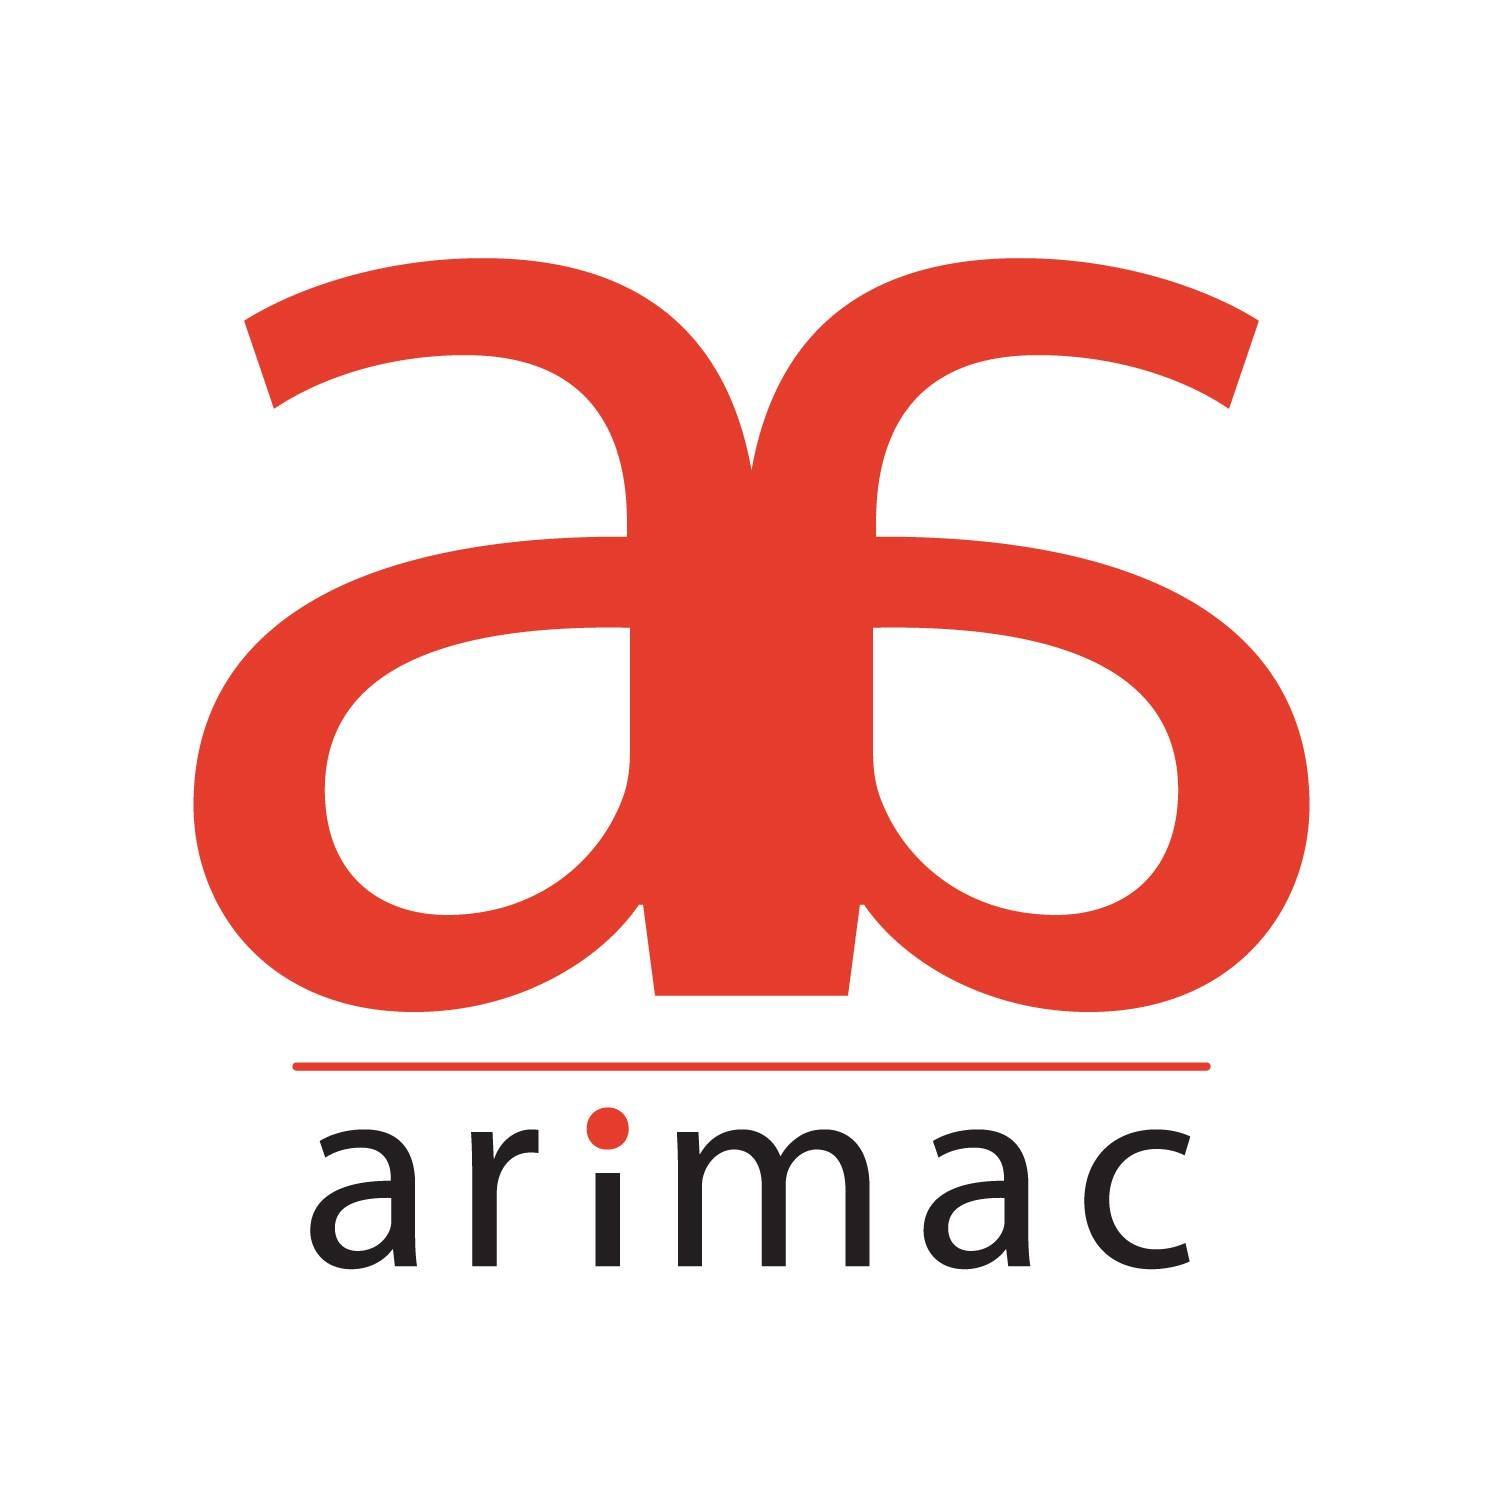
\includegraphics[width=8cm]{logo}
  \caption{Company Logo}
\end{figure}

The vision of the cheief executive officer Mr. Chamira Jayasinghe drives the company insane hights. The business was built from zero to where it is today by this truly passionate individual and the employees. 

\begin{figure}[!h]
  \centering
   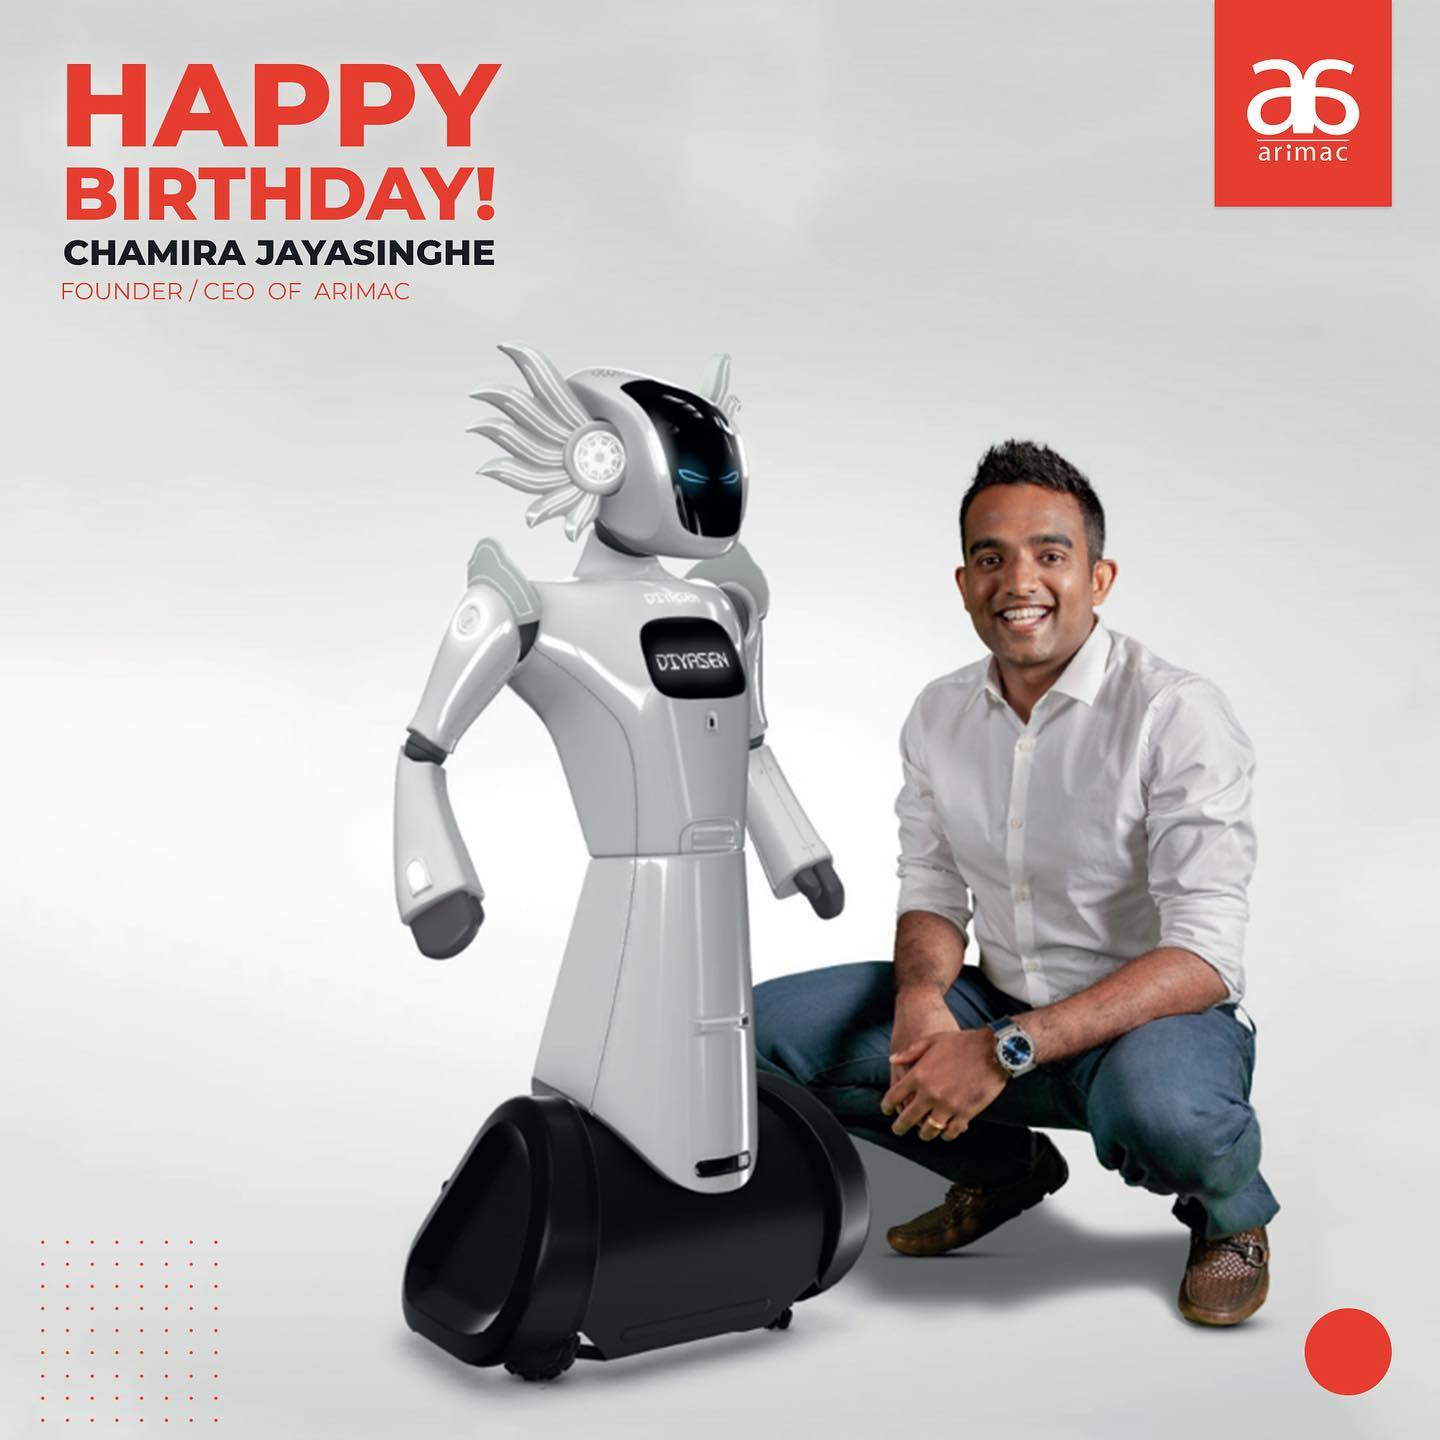
\includegraphics[width=10cm]{ceo}
  \caption{CEO Mr. Chamira Jayasinghe}
\end{figure}

\begin{figure}[H]
  \centering
   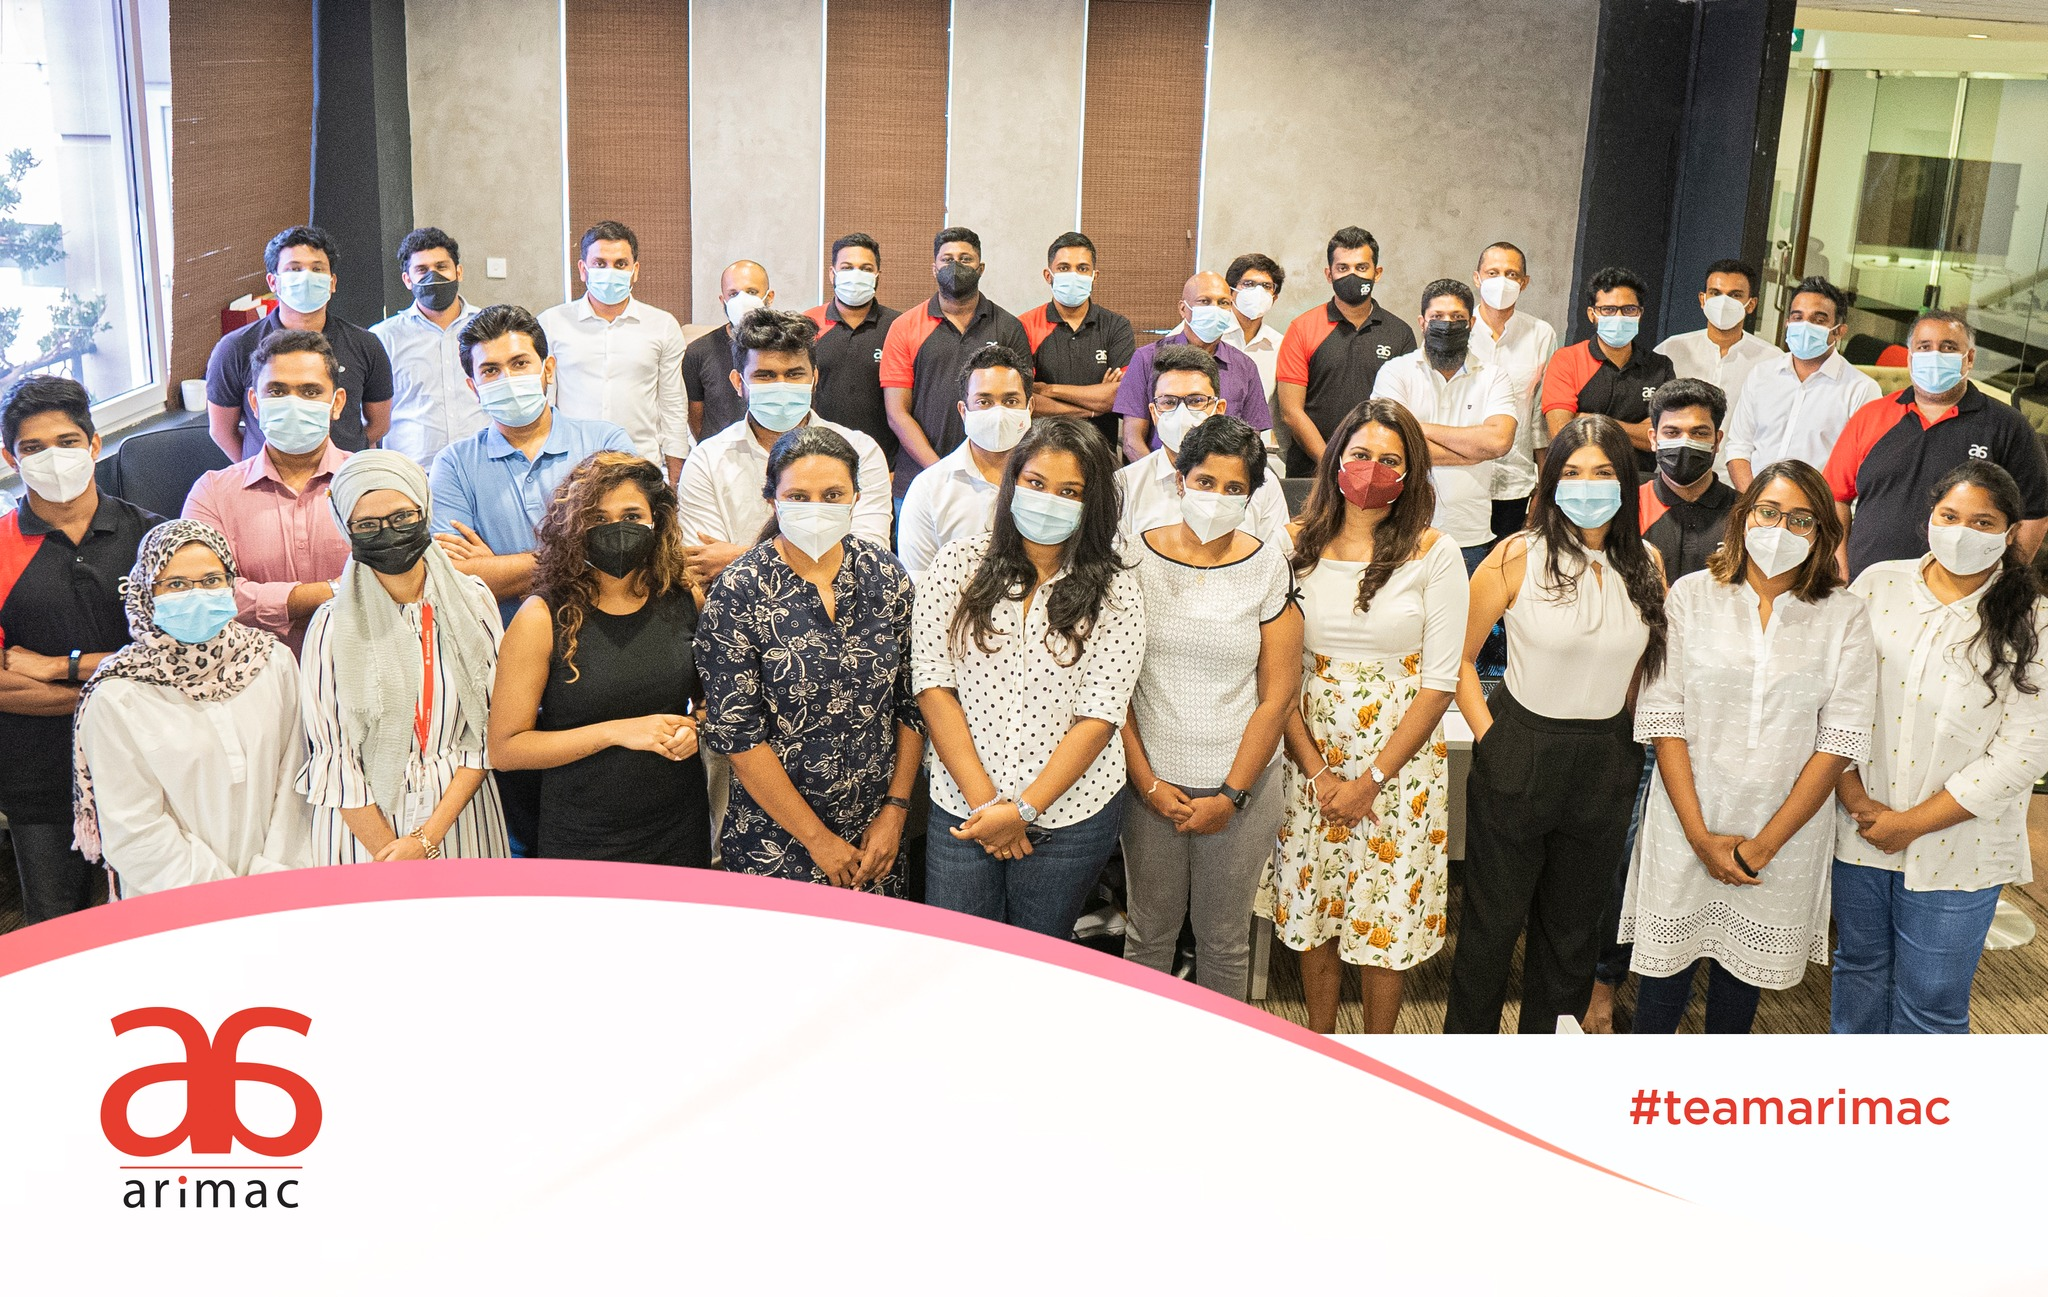
\includegraphics[width=12cm]{staff}
  \caption{CompanyTop Managementff}
\end{figure}

With more than 200 employees company is rapidly growing even during the Covid pandemic. The privately held company provides IT solution for both local and international clients with greater standards. One of the most attractive employers in the IT industry maintain their unique and pleasant company cultures to attract disruptive talents all over the country. Having said that, It is great to mention Arimac as one of them. The flat hierarchical decentralized environment makes things more convinient than anywhere else. 

\begin{figure}[H]
  \centering
   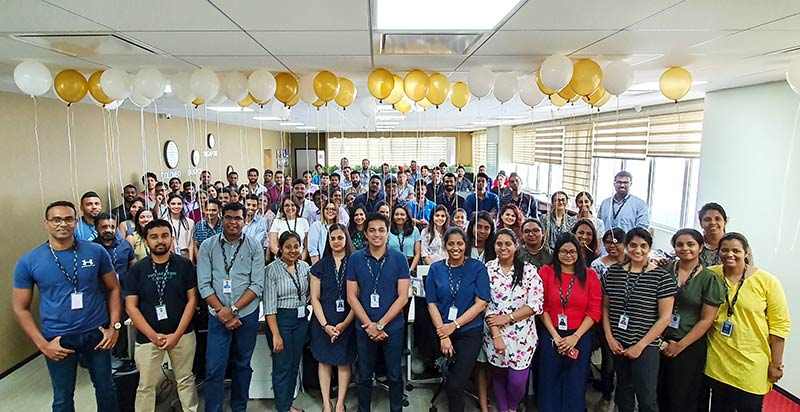
\includegraphics[width=12cm]{staff2}
  \caption{CompanyStaff}
\end{figure}

%\begin{itemize}
%  \item The nonrecursive filter obtained is of infinite length.
%  \item The filter is noncausal because the impulse response is nonzero for negative time.
%\end{itemize}

As a company of Sri Lanka, the significant achievements can be identified. Some of them are as follows,

1. First ever 3D game in Sri Lanka.
\begin{figure}[H]
  \centering
   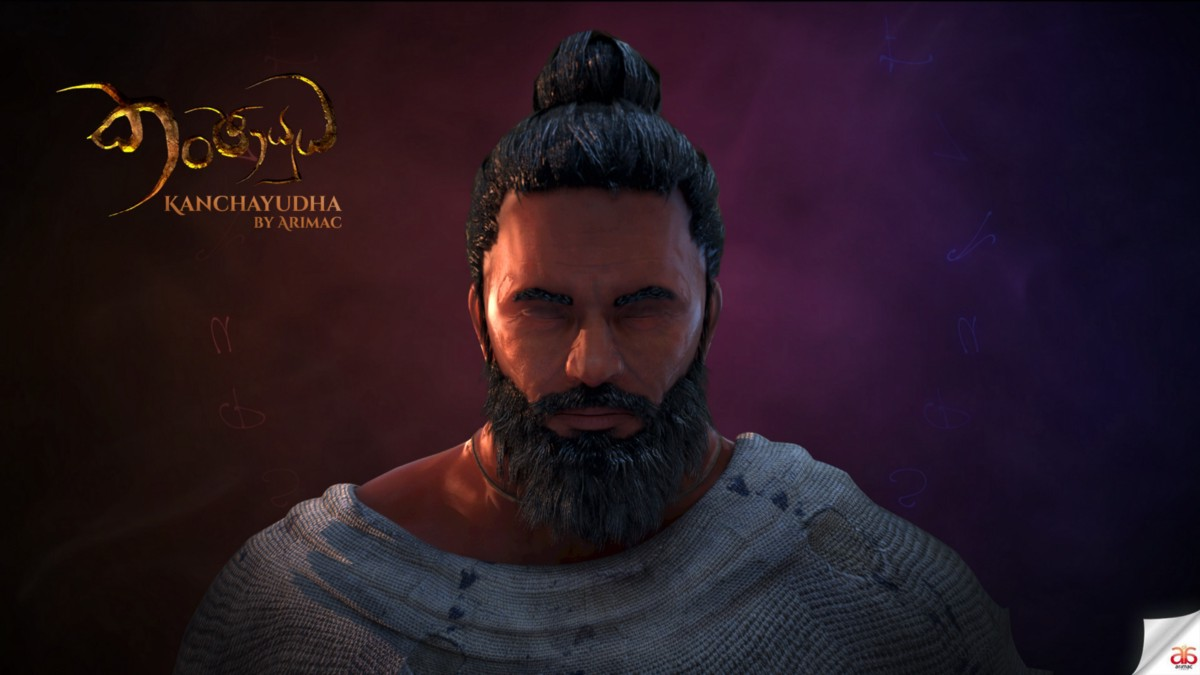
\includegraphics[width=12cm]{game}
  \caption{Kanchayudha}
\end{figure}

2. First ever Humanoid  in Sri Lanka.
\begin{figure}[H]
  \centering
   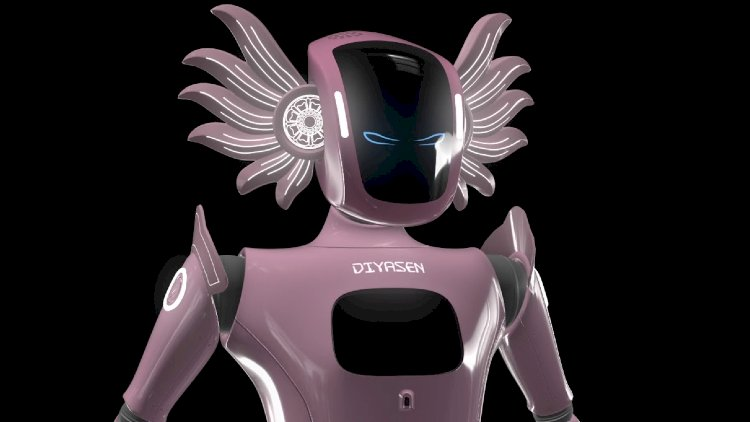
\includegraphics[width=12cm]{robot}
  \caption{Diyazen}
\end{figure}

As of now, the gaming and robotics industry is lead by the Arimac Lanka. The journey will continue. 

\chapter{Familiarization work}

\hspace{3em} Initially, the onboarding process with Arimac Lanka was completed. Basically, the required hardcopies were provided to the Human resource team. After, completeing that, first day of the internship began. Since it was the beginning of a year, the company management had organized a virtual new year celebration. At the event I got to know more about company culture and some of the coming improvemnts of the organization. The HR team and the IT support team were having most of the responsibilities with the onboarding. The companywas having their own system for track all the employees precenses, leaves and attendance to the events. The pre-created account credentials were given to me inorder to familiar with it. The IT support team sent me the all the necessary details to set up microsoft teams account. Apart from that, a personal email was generated to each employee to communicate within the team. Some of the customizations to the email signature has to be done and it was also a well documented procedure.

Later that day, the supervisor arranged a meeting with me and the fellow colleague. We introduced ourselves to the team and got to know more insights about work ethics. Next working day a group presentation was assigned to us. The main purpose of the presentation was to improve our familiarity with the humanoid robot developments and ongoing reasearch areas. We presented the findings and did a good presentation infront of our team. The next main task was to select an available humanoid robot and research about it. 

Finally, it was the time to familiar with the technical stack. The availability of a company developed pre-training repository was smoothed our work. The guided tutorial was capable of providing the required basics to us. 

After an insightful week I was in a position where I could involve with the team. Then after, all the guidance were provided to me accordingly. The supervisor gave an introduction to the project work needed to be carried out. 


\chapter{Exposure to system}


\hspace{3em} After went through a series of interviews, I got an offer letter. First time I engaged with the company system was the on-boarding process. Basically, I had to deal with the HR team. All the required details and the documents were provided. The training contract was signed accordingly.

\begin{wrapfigure}{r}{0.45\textwidth}
    \centering
    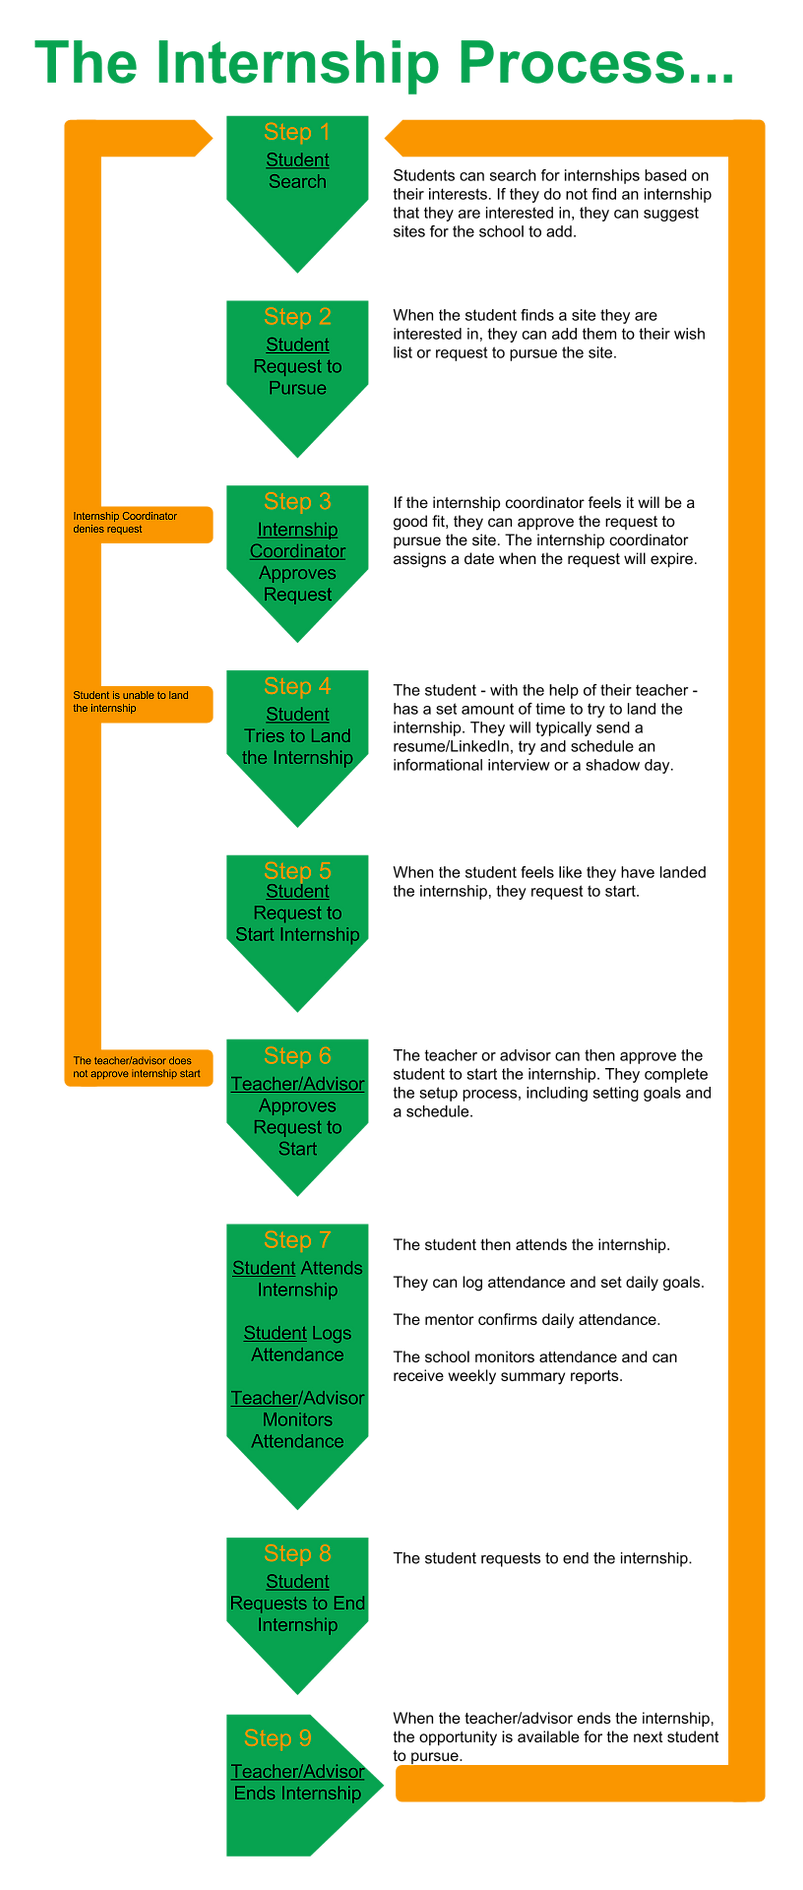
\includegraphics[width=0.2\textwidth]{intern}
    \caption{Internship Process}
\end{wrapfigure}

 Soon after, It was the time to set up my company profile. In this phase an IT support person from the company provided me all the guidance to set up my profile including the E-mail, MS teams, Jira, Gitlab and the Trello environments. Since that time I could meet the top-management people time to time in the progress reporting meetings. After receiving the second monthly allowance, I realized that there was an unexpected pay cut. So, first I contacted the HR team and got to know about the procedure that I needed to follow. Then I wrote an E-mail to the accountant and opened a request. 



Within a few working days the issue was solved. It was a quiet an experience for me as an intern. Anyways I could overcome that struggle smoothly. Finally, the off-boarding peocess was started. Again I went through the given procedure. I had to contact the all the people I dealt with before. Basically, got the approvals from respected departments and requested a service letter. 


\chapter{Project Work}

\section{Background}

The field of Robotics is a multidisciplinary and open-ended area that most of the research is going around the world. The introducing of both the computer vision and the AI into robotics has been making a huge impact in the field of Robotics for a few decades. Computer vision libraries like OpenCV and deep learning algorithms like YOLO are at the top of the list. Navigate in an unstructured environment has been challenging for robot developers, because of that vision-based obstacle avoiding and environment mapping approaches are emerging. 

\section{Objective}

One of the major concerns among the researchers is the computational cost in image processing. To overcome this, the work that has to be done is huge. In our case, the small obstacles on the floor have been a great challenge for us to smoothly navigate in an indoor environment. Most of the time, robots get blocked after collied with the small coke cans, toys and clothes on the floor. The solution for this has to be solved with the 3D depth camera sensor. Basically, the perception of the robot should be accurate with the least blind spots in order to achieve the desired outcome. 

\section{Approach}

For an autonomous operation, the system with a high accuracy real-time algorithms are optimal. Solutions such as YOLO and pre-built package find object were considered. Most of the time, computational power was the 
constraint. Therefore, the direction of the solution eventually switched to a custom 
package from scratch. The output of both RGB and depth images were taken into 
execute OpenCV operations in order to get the desired outcome. The packages 
were built to draw contours over the object using binary thresholding and OpenCV 
methods. Finally, the best possible solution was identified. A depth image 
subscriber and custom laser data publisher. The outcome was robust and scalable.

\chapter{Hands-on Experiences}

\section{Find Object 2D}

This package is open to use by anyone. The OpenCV based SURF/SIFT algorithms are used in the package. The RGB image will be the input to the package and it will be detected and published on a ROS topic with ID and position (by image pixel coordinates). First, we need to create a sample set of images to detect the features we need to identify. The implementation was successfully detected humans on the image as shown below.

\begin{figure}[!h]
  \centering
   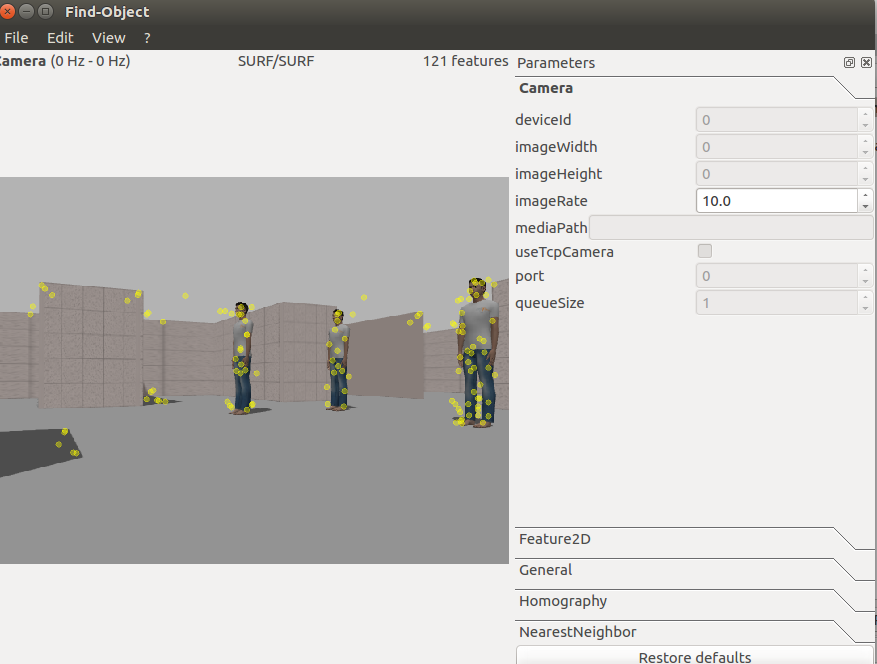
\includegraphics[width=8cm]{object_detection-fo2d}
  \caption{Find object 2D}
\end{figure}

The need is to publish the object coordinates with respect to the camera 
coordinates. Therefore, the use of Find Object package was not the solution.

\section{YOLO}

Integrating YOLOv3 into ROS is crucial for object detection to be fully utilized in 
robotics, as it allows for integration with other ROS-based capabilities that lead to exciting 
new ideas such as integration with Real-Time Appearance-Based Mapping 
(RTABMap) ROS for Simultaneous Localization and Mapping (SLAM applications. Deeplearning algorithms are highly dependent on the available computational resources. While 
training may be accomplished on more powerful hardware, issues could appear when 
implementing these algorithms on low-SWaP platforms. Specifically, if many processes 
with high memory usage are running simultaneously, darknet Ros may not perform 
optimally.
The integration was successful. Using the pre-trained models, the darknet was able 
to identify the object and draw a box over it in an appropriate manner. The small obstacles 
could have been identified with a new model which can be trained using the CUDA. The 
low frame rate and the significantly lower frame rate caused regret this solution for further 
development. 

\begin{figure}[!h]
  \centering
   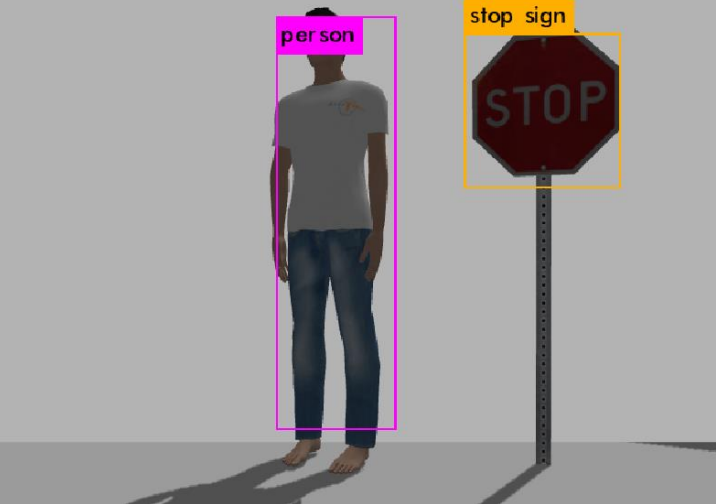
\includegraphics[width=12cm]{yolo}
  \caption{YOLO output}
\end{figure}

\section{Object Recognition Custom Package}

\subsection{RGB}

The navigation in an unstructured environment is quite difficult for a humanoid robot 
as it may collide with moving objects or small objects on the floor. To overcome this 
difficult challenge, the use of computer vision would be a great solution. 
The small objects on the floor should differentiate from the floor. To do that, the 
custom package subscribed to the color image published by the Kinect depth camera. 
Then the image is converted into OpenCV processible type. The RGB8 image then 
converted into grayscale format. From that, a proper threshold can be identified in order to 
create a binary image. The objects are identified and bounding objects can be drawn 
around them.

\begin{figure}[!h]
  \centering
   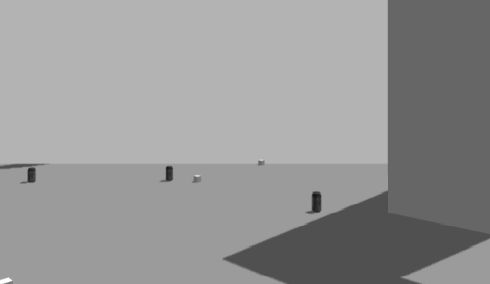
\includegraphics[width=15cm]{gray}
  \caption{Gray Image}
\end{figure}

\begin{figure}[!h]
  \centering
   
\includegraphics[width=15cm]{binary}
  \caption{Binary Image}
\end{figure}

\begin{figure}[!h]
  \centering
   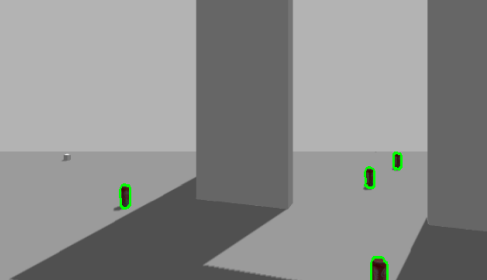
\includegraphics[width=15cm]{detected}
  \caption{Objects Detected}
\end{figure}

\subsection{Depth}

Depth image manipulation is also possible with the OpenCV library. To do 
that we have to have a bridge between Ros topic and the OpenCV. As we did for the 
color image, we could write a subscriber. As the next step, I tried to display the 
distance to an object using the custom package. If an object is detected, the 
distance for the object from the camera frame will be displayed in meters. It was 
successful and the results are as follows.

\begin{figure}[!h]
  \centering
   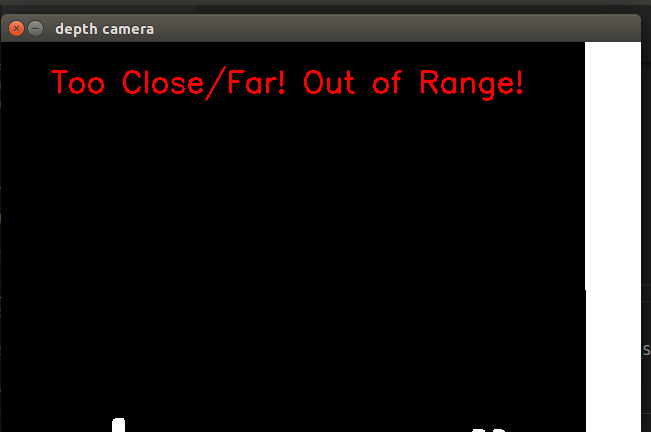
\includegraphics[width=15cm]{depth_output}
  \caption{Not Detected}
\end{figure}

\begin{figure}[!h]
  \centering
   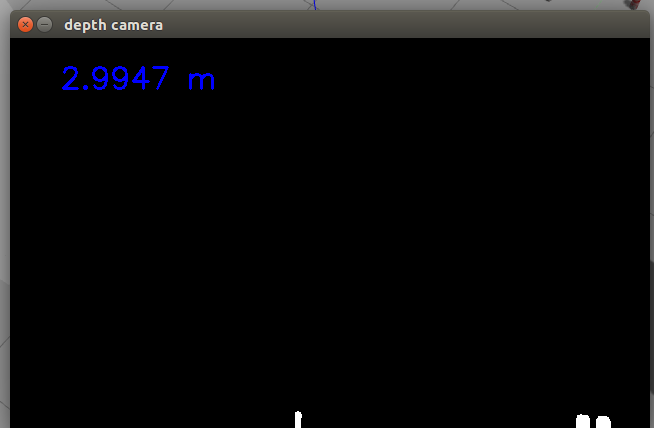
\includegraphics[width=15cm]{depth-out-dist}
  \caption{Distance Display}
\end{figure}

As the final step, a custom laser message should be created. Then the created laser 
message should publish to the ROS needed to be done.

\section{ Git and Gitlab}

\subsection{Git}
To start with the development task, I went through the Git tutorials that I could learn about the versioning system.The SSH communication was done using private and public key pair.  From the "git initiate to merging" was studied and use with the project. 

\begin{figure}[H]
  \centering
   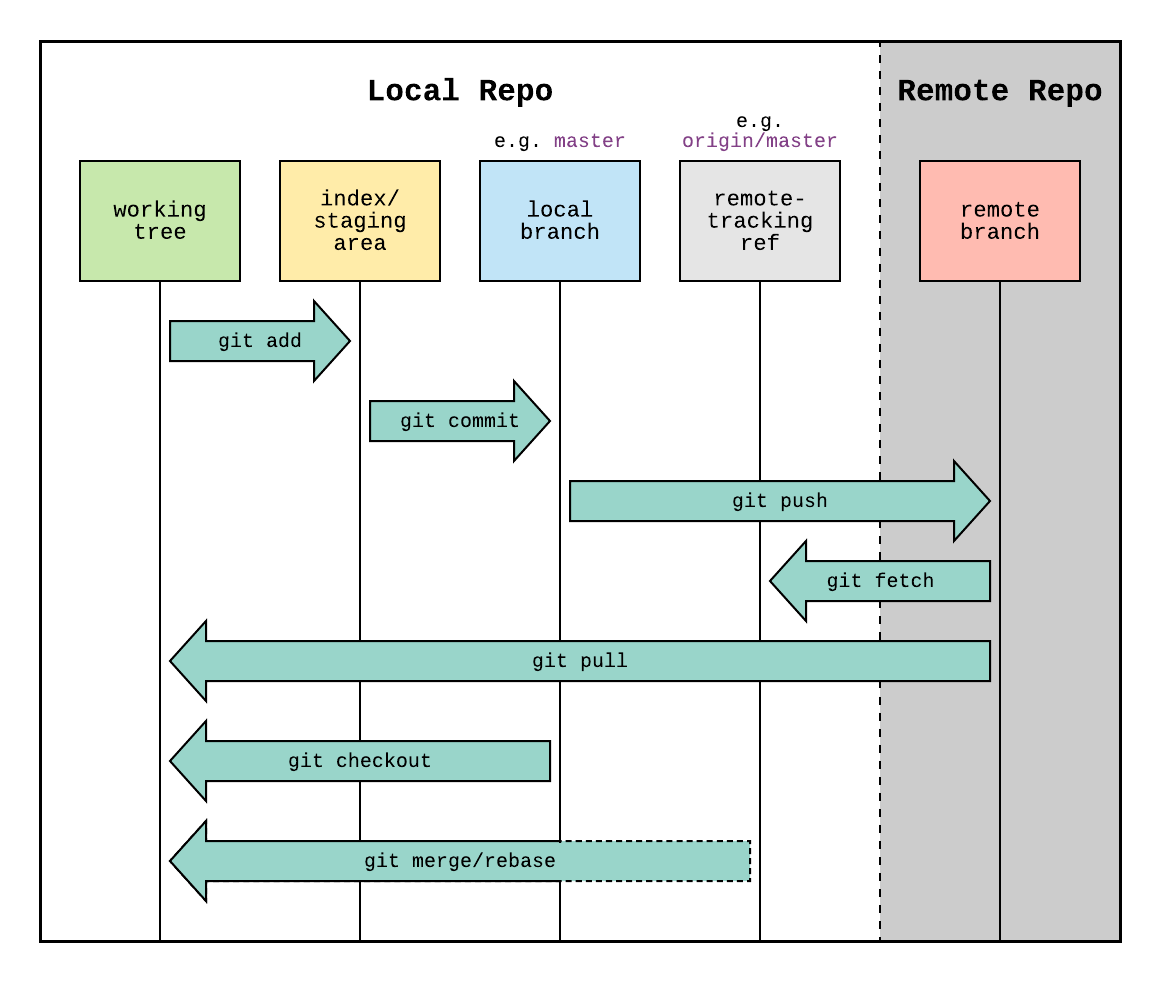
\includegraphics[width=15cm]{git}
  \caption{Git Explain}
\end{figure}


\subsection{Gitlab}
All the work were managed on Gitlab private workspace. Basically, the Gitlab private workspace consists of well documented robot simulation up until the Autonomous navigation. The repository was forked into our development projects and testings were done in there. Eventually, I our well organized and documented branches were merged and requested to merge accordingly. This is the most common and appropriate approach in software development. 

Apart from that, we use Microsoft visual studio code as our editor. Having a lot of extentions and terminal accessibility, The editor was able to enhance the comfort of the work. 

\section{ Jira and Project Management}

The project management helps the organization to make the best from their talents and time. The team was following an agile methodology. The outcome based system directly monitor the progress using tools such as Jira. The daily updates to the Jira board should be completed after the daily scrum. It enabled me to stick with the development team and compare my work with others. 

\begin{figure}[H]
  \centering
   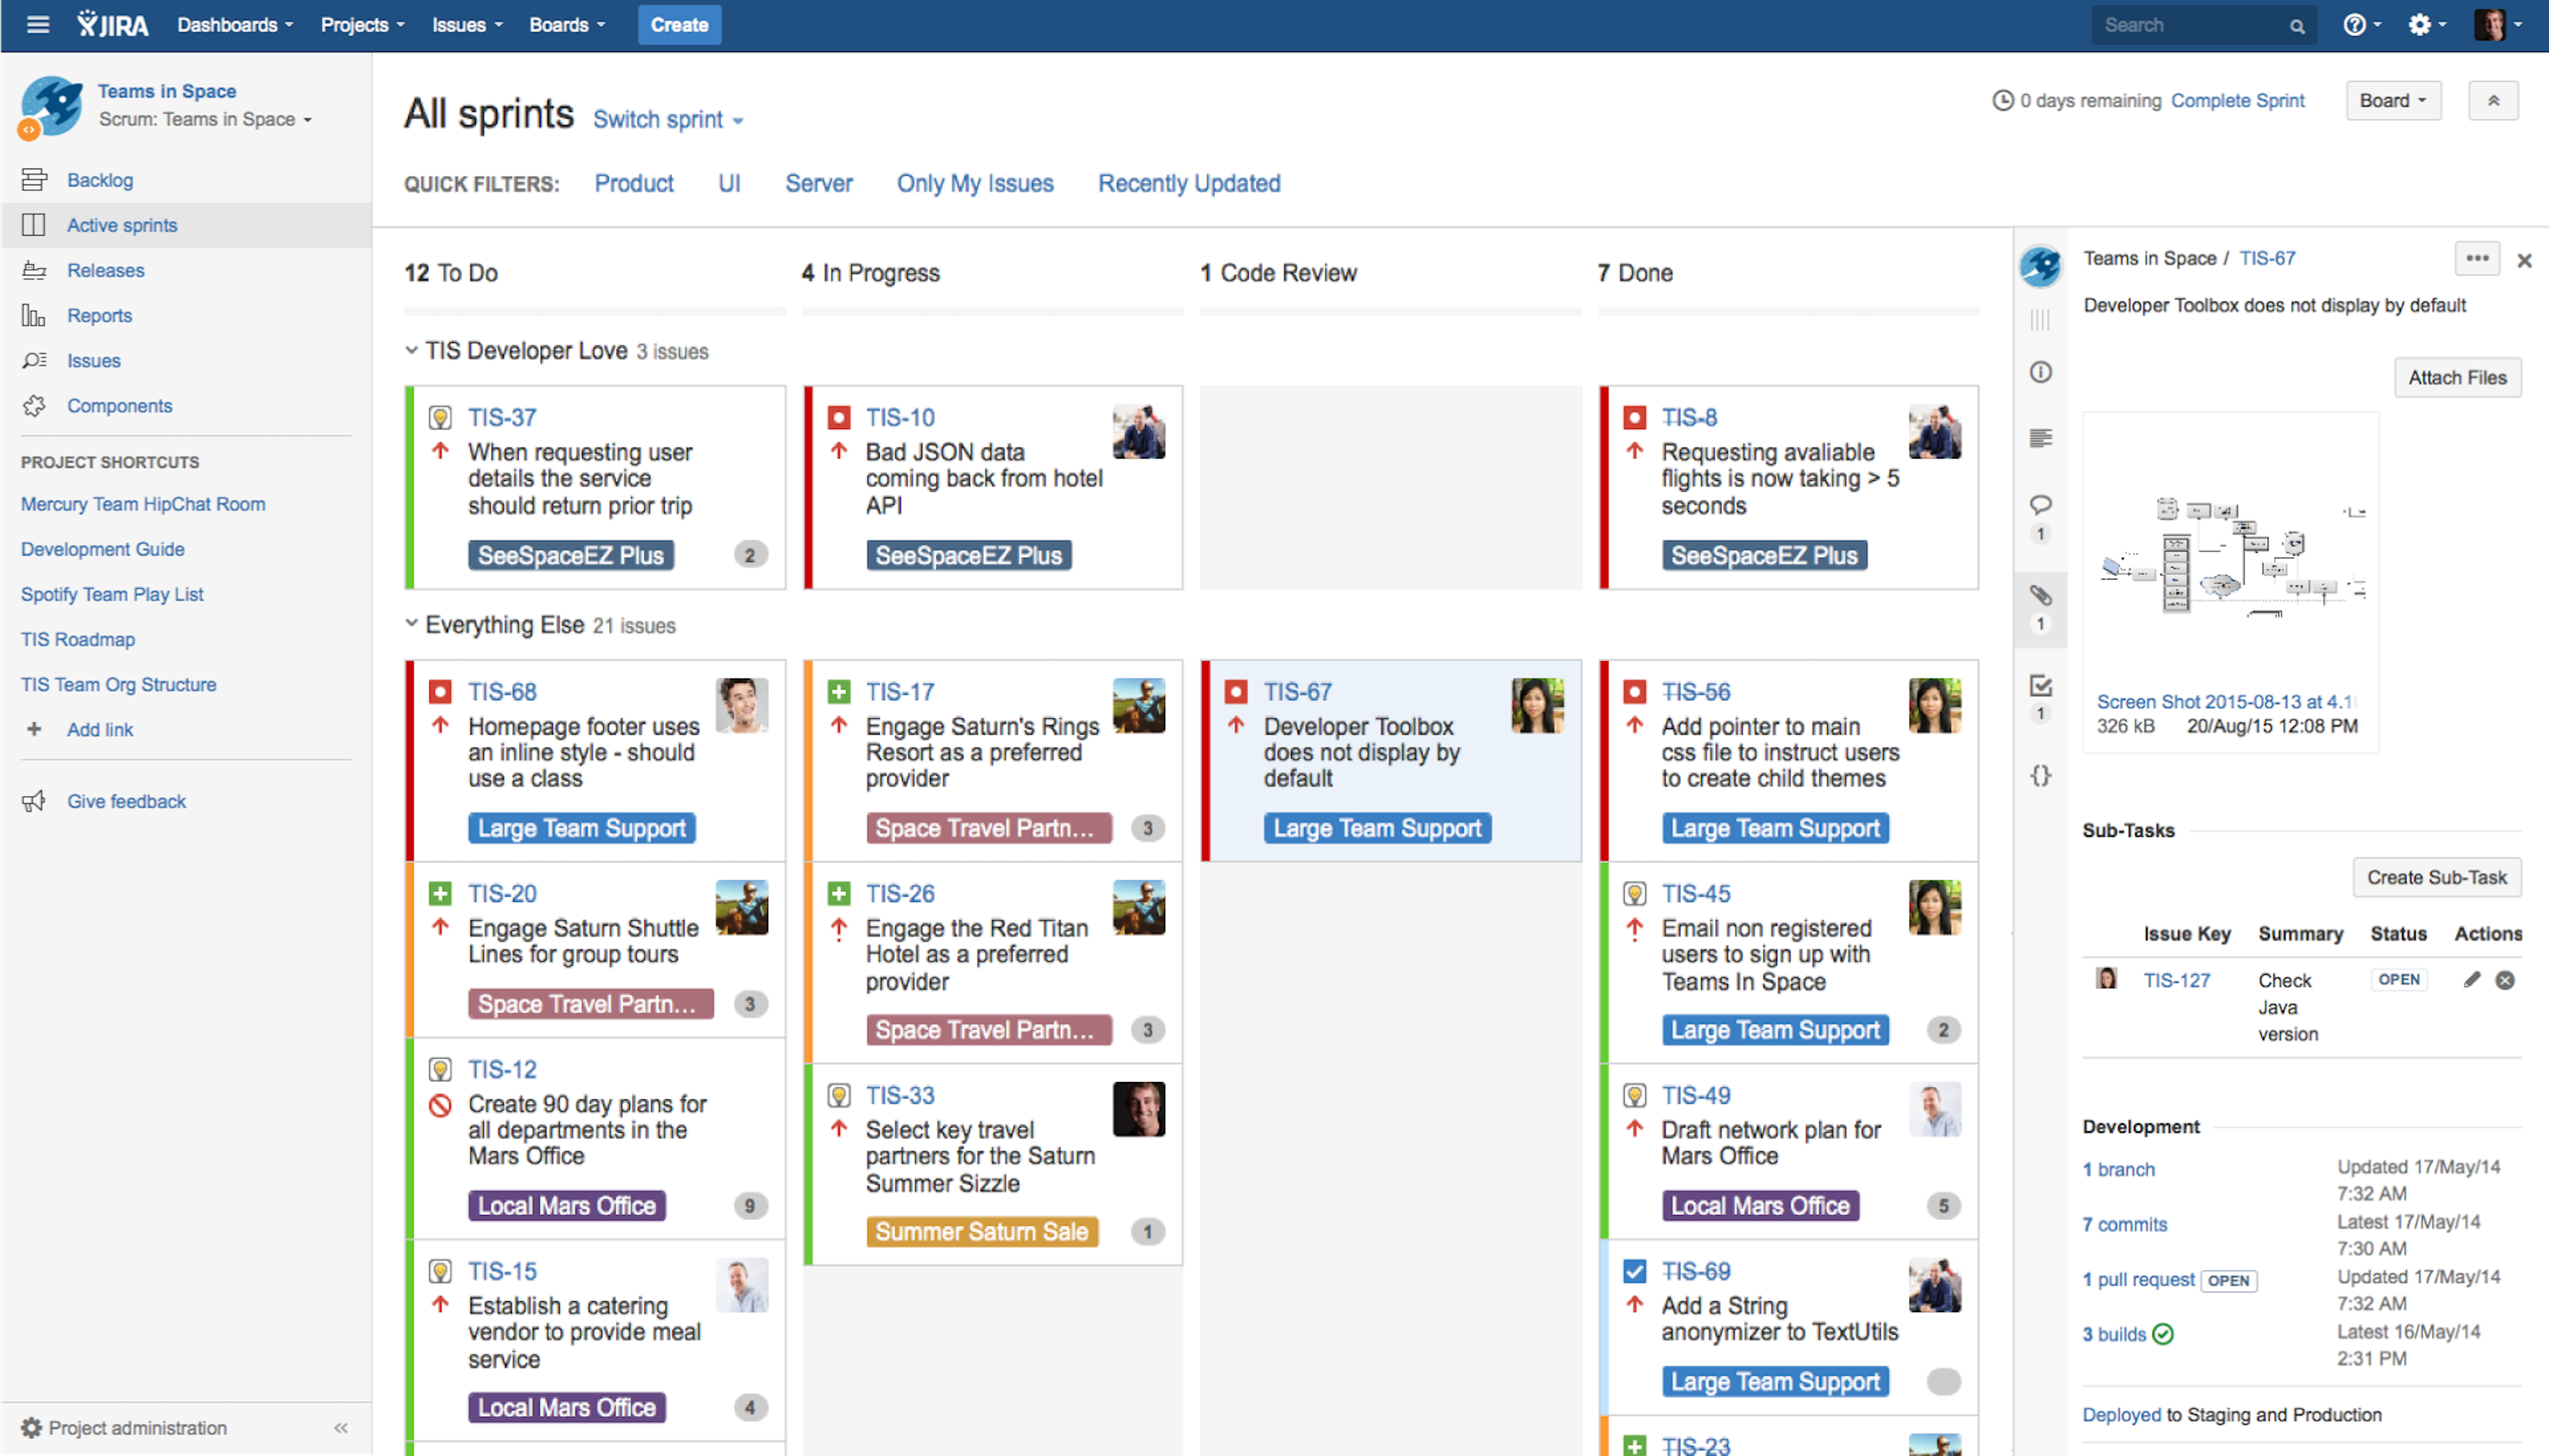
\includegraphics[width=15cm]{jira}
  \caption{Jira agile board}
\end{figure}


\chapter{Soft skills development}

During the internship I got a lot of opportunities to interact with people. Soft skills are non-technical skills that relate to how I work. They include how I interact with colleagues, how you solve problems, and how you manage your work.

\section{Work Ethic}
As an Intern Electronic Engineer, it was my first exporsure to the industry. There are actually, a set of dos and don'ts that we should be aware of. Everytime I made a mistake, the team members were always there to support me. At one time, I just changed a code script on my own. Lately, I identified my mistake and corrected it. The help I received from my team to undo my mistake was massive. The industry is moving forward with the collaborativeinnovations. So, It's good to discuss and learn from others.  

\section{Time management}
Time management was a challenge for me since I started working on projects. The prevailing situation cut out a significant portion of day and night time due to lack fuel supplies for the power plants. To overcome this unavoidable and significant consequnces effectively was my target. Becase of that I did my work even in the late nights and was able to stick with the timeline of the project team. 

\section{Networking}
The friendly and flat hierarchy of the company helped me a lot to meet new people and even connect with them in platforms like LinkedIn. It was great and I took all the opportunities to make good connections. Hopefully, having a wider network of professionals with I will be rewarding. More than 70 percent of hiring happen as internal hirings. So, a new space of employment opportunities will open with the networking. 

\section{Creative Thinking}
The project team and the supervisor had a growth mindset and always let me to try out different experiments and learn from them. The freedom I needed to unleash my true potential was there. Always be appreciated the work I did on my own. 

\section{Team work}
Since the begining of the internship I got paired with the fellow interns and worked together to fulfil tasks. A presentation about Humanoid Robots was at the beginnig. Eventually, more advance and challenging group works were there. Working with a team was much interesting and efficient. I felt that I could easily, find solutions to arising problems with the support of others. We had several meetings on our own and discuss our problems. One thing that I was impressed by is while completing a task I got a problem which cost me around eight working hours, but with the team support, just a simple set of codes solved it quickly. 

\section{Communication Skills}

Throughout the internship period of Arimac, I could enhance my communication skills time to time. Starting from the interwieving and on boarding, the opportunity was always there until I got my service letter. The format of a business e-mail was something that I did't know, but while working with them I caught some insights on the domain and could able to compose a formal e-mail according to the need. Presentation skills were something that I was not very good with. Eventually, by practicing and delivering presentations, I could collect the all basic skills that required to deliver and prepare a presentation. Apart from that, negotiation and general speaking skills were improved. 

\chapter{ SWOT Analysis }
\hspace{3em}SWOT analysis is an analytical method/tool which is used to identify and categories significant internal (Strengths and Weaknesses) and external (Opportunities and Threats) factors faced either in a particular arena, such as an organization, or a territory, such as a region, nation, or city.
It provides information that is helpful in matching the firms’ resources and capabilities to the competitive environment in which it operates and is therefore an important contribution to the strategic planning process. It should not be viewed as a static method with emphasis solely on its output, but should be used as a dynamic part of the management and business development process. Sri Lankan IT industry is the most significant and dynamic contributor to Sri Lanka’s economy. It has the potential of becoming one of the leading service providers in the world. 


\begin{table}[!h]
\centering


 \begin{tabular}{||p{0.4\textwidth}|p{0.5\textwidth}||}
 \hline
 Opportunities & Threats\\ [0.5ex] 
 \hline\hline
 Have wide range of product and services, can share service of each sector & Have to compete with many other IT companies. \\ 
 \hline
Internationally recognized company, Have larger potential market for the products& Government policies may some time effect in drawn back of the IT services industry and product manufacturing.  \\
 \hline
Easy to introduce new products to the market  &   \\ [1ex]
\hline
 \end{tabular}
\caption{External Opportunities and Threats.}
\label{tab:table1}
\end{table}

\begin{table}[!h]
\centering
 \begin{tabular}{||p{0.4\textwidth}|p{0.5\textwidth}||}
 \hline
 Strenghts &  Weaknesses \\ [0.5ex] 
 \hline\hline
 Availability of skilled labor & Increasing cost of labor and availability of employment in other industries and foreign employment opportunities. \\ 
 \hline
 Educated and trainable work force & Constant power interruptions reduce productivity.  \\
 \hline
Management of production capacity  & Lack of available equipments and maintanance.  \\  
 \hline
Partnered with best international Players & Increasing taxes and import restrictions.\\
 \hline
Well established sales and distribution system &   \\
 \hline
Ability to handle high volume orders &   \\ [1ex]
\hline
 \end{tabular}
\caption{Internal Strengths and Weaknesses.}
\label{tab:table1}
\end{table}


\chapter{Conclusion}
\hspace{3em} The Industrial Training I completed with the Arimac Lanka Robotics team is one of the most valueble opportunities in my carieer. As an Electronic and Telecommunication Engineering undergraduate in University of Moratuwa, I could enhance my almost every technical and personal skills with the immense support of so many people. In my opinion the internship could have been more exciting without the prevaling situation of the country. I recommend Arimac Lanka as a great place to complete your internship. They provide you the most valueble skills and experience. The work environment, ethics and rules they follow are best suits for a student growth as a youngster to the Industry. 

With more than 200 employees company is rapidly growing even during the Covid pandemic. The privately held company provides IT solution for both local and international clients with greater standards. One of the most attractive employers in the IT industry maintain their unique and pleasant company cultures to attract disruptive talents all over the country. Having said that, It is great to mention Arimac as one of them. The flat hierarchical decentralized environment makes things more convinient than anywhere else. 

The outcome based architecture encourage us to deliver more robust and innovative solutions. The appreciation get from the supervisors and the rest of the team mostly motivated me to achive my project goals. Everyday scrums were also helped me to keep in track with the project team. Because of that, I pushed my self to the limits and reched to comparatively high standards as an Intern. Opportunity to build good relationships with the industry experts and the top level managers would be appriciated. During the internship I got a lot of opportunities to interact with people. Soft skills are non-technical skills that relate to how I work. They include how I interact with colleagues, how you solve problems, and how you manage your work. Almost every aspects of the work ethics and the policies were maintained accordingly, So the upskilling is smmoth and crystal clear. \\\\

\centering
Thank You!




\medskip

\appendix
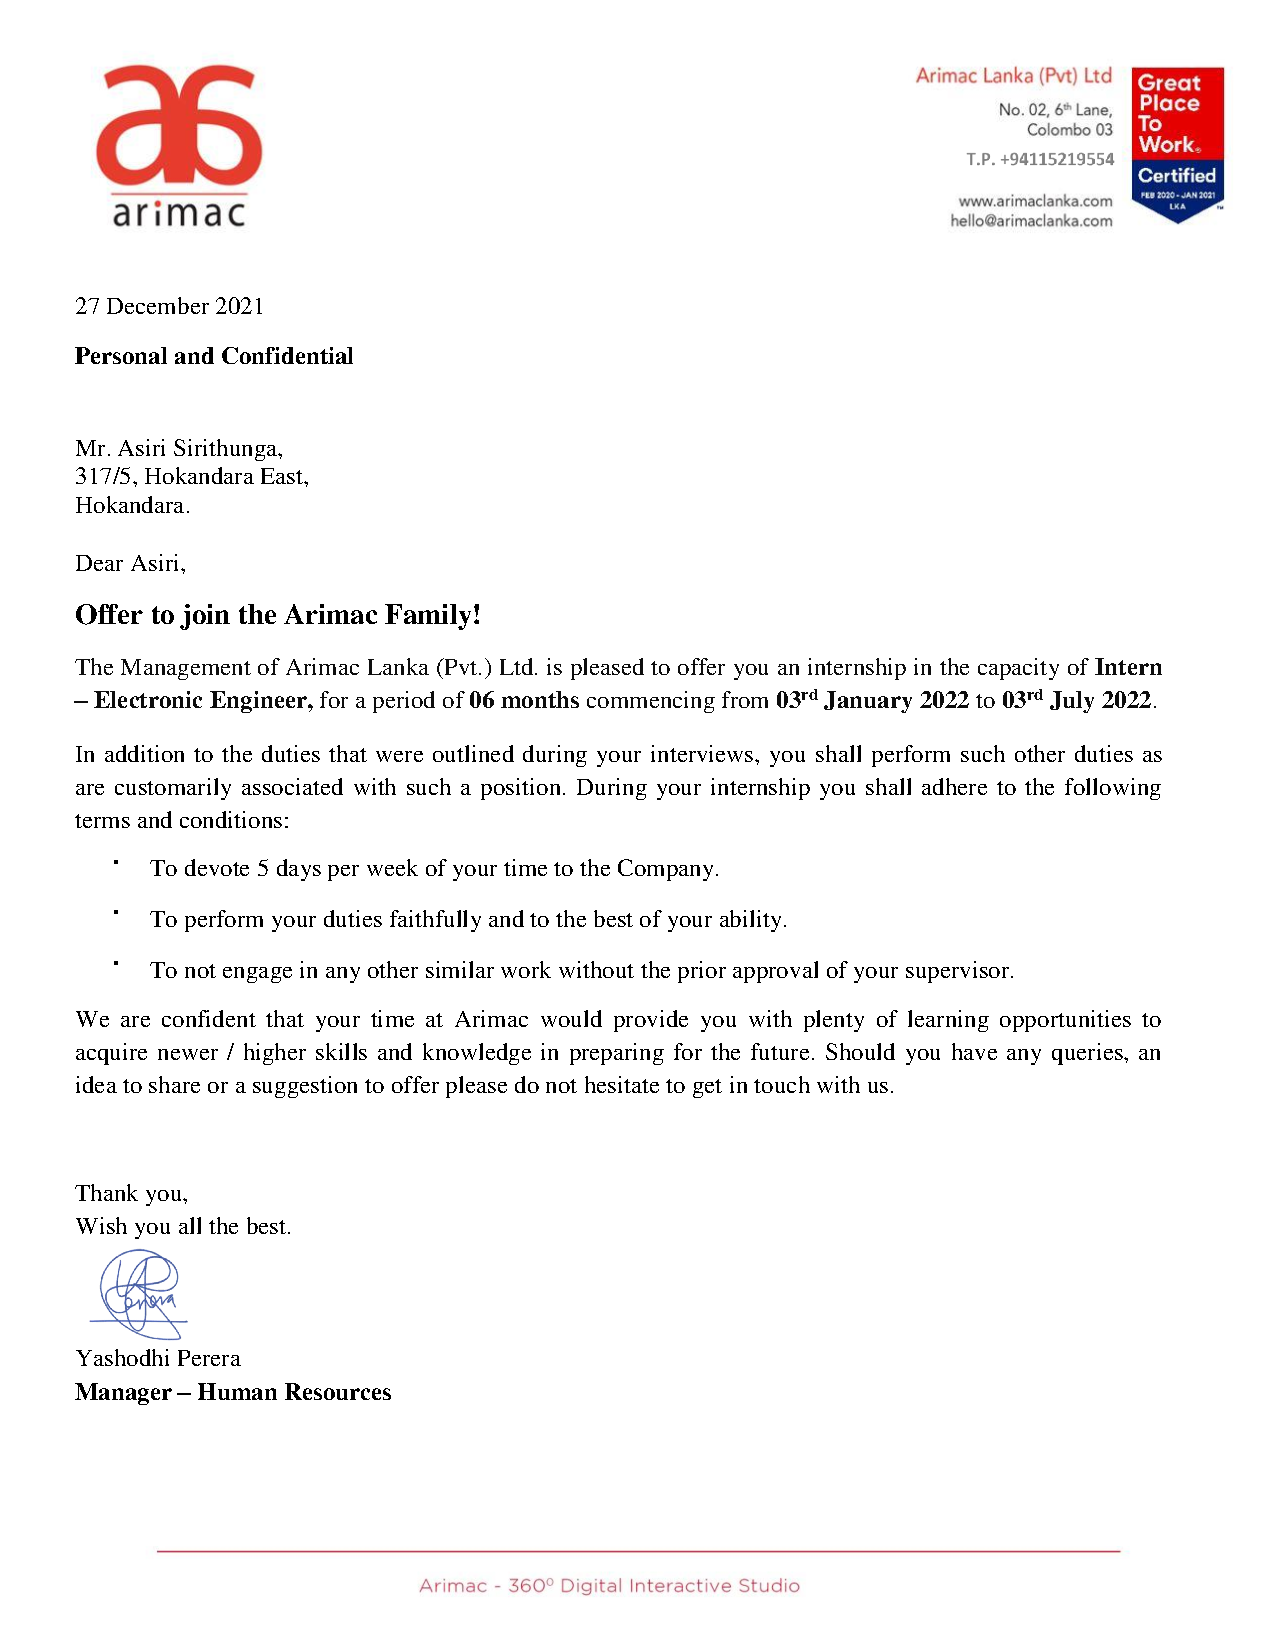
\includepdf[width=1\textwidth,pages=-,pagecommand=\thispagestyle{plain}]{Offer letter -Asiri Sirithunga.pdf}
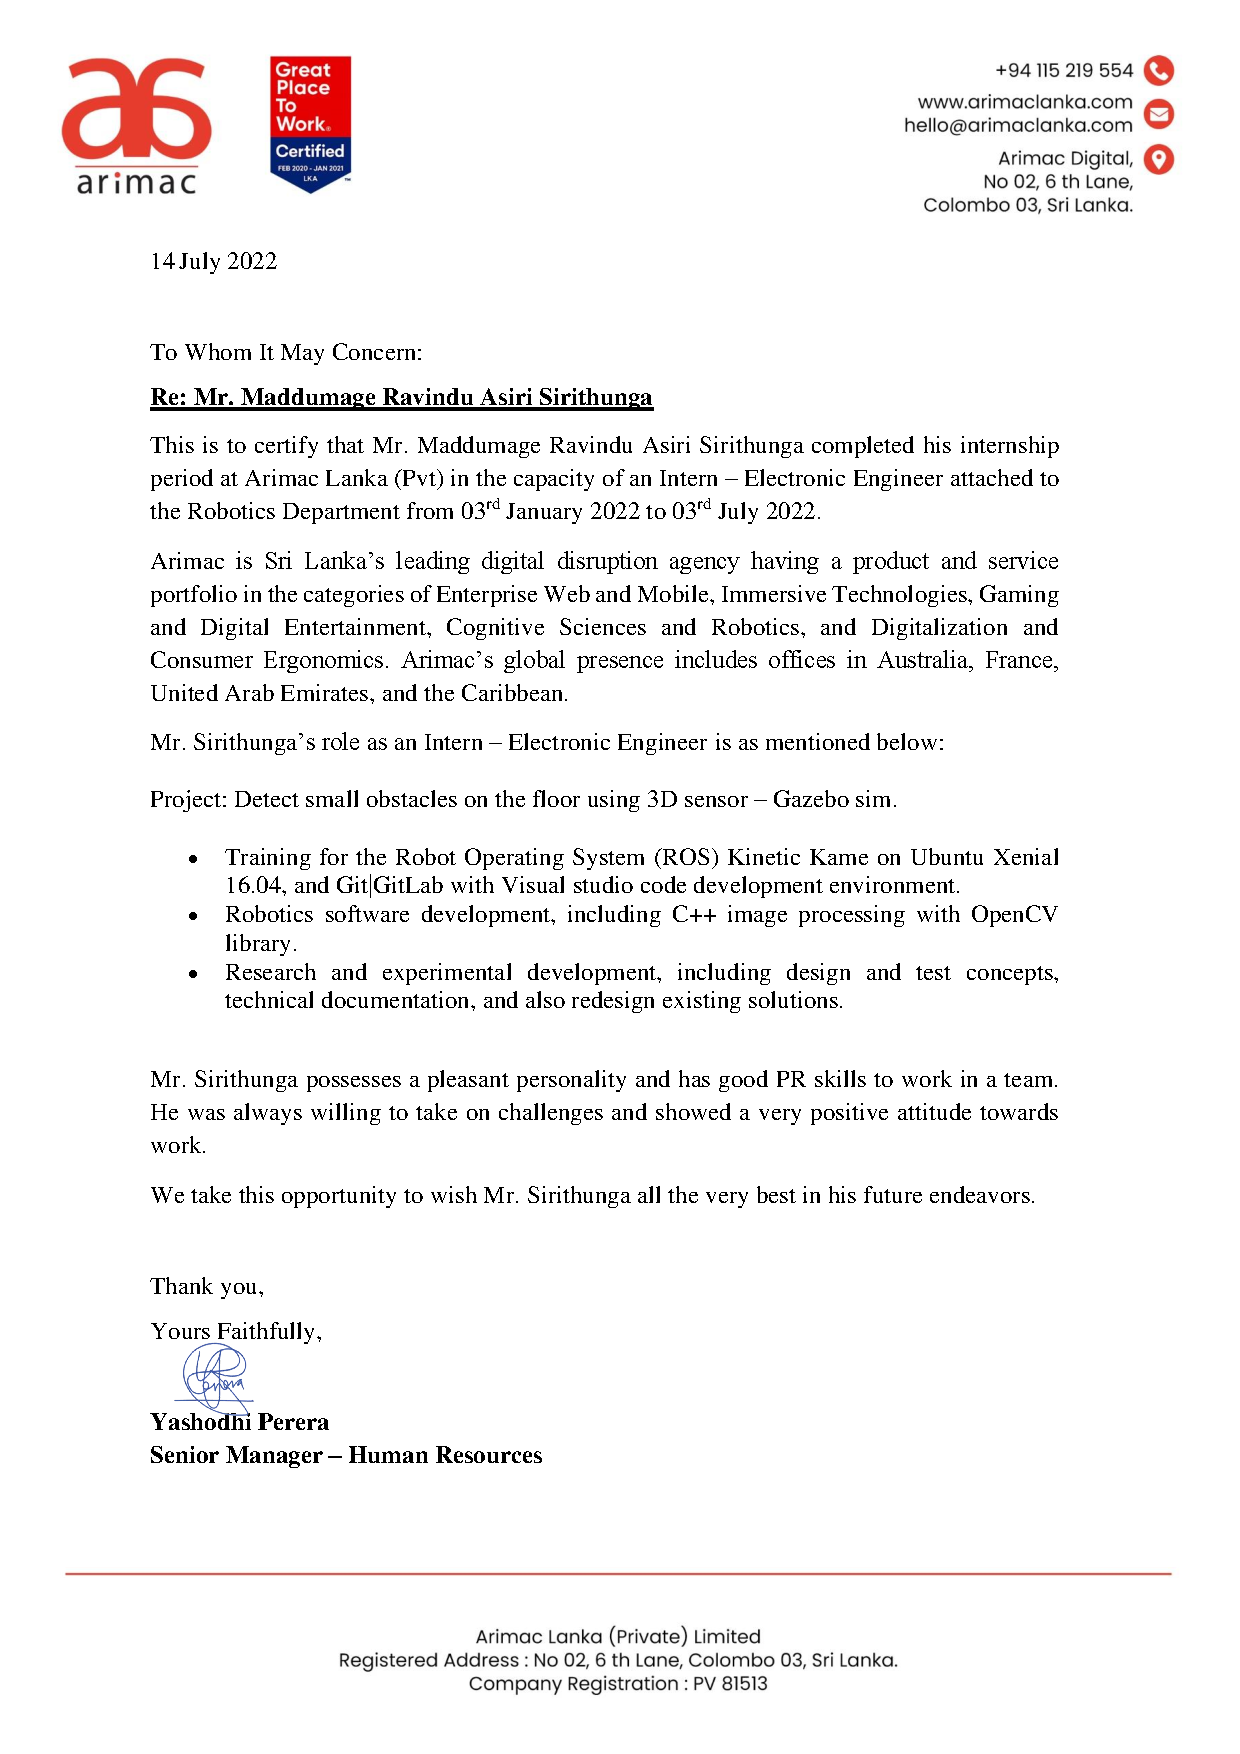
\includepdf[width=1\textwidth,pages=-,pagecommand=\thispagestyle{plain}]{Service Letter - Asiri Sirithunga.pdf}

\begin{thebibliography}{9}
%book
\bibitem{Cacace, J. and Joseph, L. (2018).} 
Cacace, J. and Joseph, L. (2018). 
\textit{Mastering ROS for Robotics Programming, 
Second Edition: Design, build, and simulate complex robots using the Robot 
Operating System, 2nd Edition. [online] Open WorldCat. Birmingham: Packt 
Publishing. }
Available:  https://www.worldcat.org/title/mastering-ros-for-robotics-programming-second-edition-design-build-and-simulate-complex-robots-using-the-robot-operating-system-2nd-edition/oclc/102818037/

\bibitem{Vines} 
Vines (n.d.). 
\textit{Getting RGB and Depth image from Azure Kinect in ROS. [online] 
Vines’ Note.}
Available: https://vinesmsuic.github.io/2021/01/08/azure-kinect-ros-basic/


\bibitem{Ieee Paper} 
S. Zhao and S. -H. Hwang
\textit{"Path planning of ROS autonomous robot based on 2D lidar-based SLAM," 2021 International Conference on Information and Communication Technology Convergence (ICTC), 2021, pp. 1870-1872, doi: 10.1109/ICTC52510.2021.9620783.Abstract: Indoor robots are more and more widely used, and their path planning directly affects traverse efficiency and quality, which has always been a hot research topic. Excessive requirements for sensor accuracy and accuracy may reduce the adaptability of path planning or cause unacceptable costs. Based on the analysis of the path planning requirements of the indoor robot, this paper proposes a ROS path planning method based on 2D Lidar-based SLAM. The algorithm is simple and effective. In the simulation test, the robot has a high coverage of the entire area and strong environmental adaptability. }
Available: https://ieeexplore.ieee.org/stamp/stamp.jsp?tp=\&arnumber=9620783\&isnumber=9620211


%site
\bibitem{ROS Documentation} 
ROS Documentation
\\\texttt{https://docs.ros.org/}

\bibitem{Gitlab Documentation}
 Documentation for GitLab Community Edition, GitLab Enterprise Edition, Omnibus GitLab, and GitLab Runner.
\\\texttt{https://about.gitlab.com/handbook/documentation/}

\bibitem{Sudo Null} 
Company, S.N. (n.d.). Sudo Null - Latest IT News. [online] SudoNull. 
\textit{Detection and recognition of objects from the camera in ROS.}
Available: https://sudonull.com/post/14732-Detection-and-recognition-of-objects-fromthe-camera-in-ROS-using-the-package-find-objehttps://sudonull.com/post/

\bibitem{Ieee Paper 2} 
S. Gatesichapakorn, J. Takamatsu and M. Ruchanurucks
\textit{"ROS based Autonomous Mobile Robot Navigation using 2D LiDAR and RGB-D Camera," 2019 First International Symposium on Instrumentation, Control, Artificial Intelligence, and Robotics (ICA-SYMP), 2019, pp. 151-154, doi: 10.1109/ICA-SYMP.2019.8645984.Abstract: This paper presents an implementation of autonomous mobile robot with the robot operating system (ROS). The system utilizes 2D LiDAR and RGB-D camera with ROS 2D navigation stack, with low power consumption and inexpensive onboard computer. Safe to property and human is of priority. Regarding software, we use official ROS packages with minimal default parameter changes. For hardware, the limitation of equipment and system setting are among challenges. Our proposed systems can perform navigation with dynamic obstacle avoidance capability. The Contribution of this paper is two system setups of ROS navigation stack are proposed. The first system is implemented on Raspberry Pi 3 using 2D LiDAR only. The second system is implemented on Intel NUC using 2D LiDAR and RGB-D camera. To evaluate the performance, usability testing was performed in multiple experiments. Our experiment results show that the robot can avoid objects in their path, or stop in case of unavoidable. Discussion of problems and solutions are presented after the experiment results. }
Available: https://ieeexplore.ieee.org/stamp/stamp.jsp?tp=\&arnumber=8645984\&isnumber=8645979


%\bibitem{Ieee Paper 3} 
%D. Maier, A. Hornung and M. Bennewitz
%\textit{"Real-time navigation in 3D environments based on depth camera data," 2012 12th IEEE-RAS International Conference on Humanoid Robots (Humanoids 2012), 2012, pp. 692-697, doi: 10.1109/HUMANOIDS.2012.6651595.Abstract: In this paper, we present an integrated approach for robot localization, obstacle mapping, and path planning in 3D environments based on data of an onboard consumer-level depth camera. We rely on state-of-the-art techniques for environment modeling and localization, which we extend for depth camera data. We thoroughly evaluated our system with a Nao humanoid equipped with an Asus Xtion Pro Live depth camera on top of the humanoid's head and present navigation experiments in a multi-level environment containing static and non-static obstacles. Our approach performs in real-time, maintains a 3D environment representation, and estimates the robot's pose in 6D. As our results demonstrate, the depth camera is well-suited for robust localization and reliable obstacle avoidance in complex indoor environments.
%}
%Available: https://ieeexplore.ieee.org/stamp/stamp.jsp?tp=\&arnumber=6651595\&isnumber=6651490


\end{thebibliography}

\end{document}